\chapter{Descriptors (falta quillbot'ar este cap todo)}
\label{cha:descriptors}

In this work, we first examined the state-of-the-art in computationally predicting ... and then comprehensively assessed the predictive power of eight traditional machine learning methods and 17 feature types often used in prior research.

Based on the sequence and physicochemical characteristics, we created and evaluated a total of 17 different kinds of features.

\section{Psycho chemical}

\subsection{Length}

Length descriptor is a simple descriptor that calculates the length of a sequence.

\subsection{GC Content}

\gls{GC} content feature enconding represents the quantity of guanine and cytosine nucleotides in a sequence. It can be calculated as follows:

\begin{equation}\label{eq:gc_content}
    x = \frac{N_{(C)} + N_{(G)}}{N}
\end{equation}


where $N_{(C)}$ donates the number of the nucleotide C in the sequence, $N_{(G)}$ the number of the nucleotide G and $N$ the length of the sequence.

\subsection{AT Content}

\gls{AT} content feature enconding represents the quantity of adenine and thymine nucleotides in a sequence. It can be calculated as follows:


\begin{equation}\label{eq:at_content}
    x = \frac{N_{(A)} + N_{(T)}}{N}
\end{equation}

where $N_{(A)}$ donates the number of the nucleotide A in the sequence, $N_{(T)}$ the number of the nucleotide T and $N$ the length of the sequence.

\section{Nucleic acid composition}

\subsection{Nucleic Acid Composition}

As one of the commonly used methods to represent \gls{DNA} sequences, the \gls{NAC} encoding [25, 26] reflects the nucleotides frequencies of the sequence. The frequencies of all four natural nucleotides ('A', 'C', 'G' and 'T') can be calculated as:

\begin{equation}\label{eq:NAC}
    f(i) = \frac{N_{(i)}}{N}, i \in \left\{A,C,T,G\right\}
\end{equation}

where $N_{(i)}$ donates the number of nucleotide type and $N$ represents the length of a \gls{DNA} sequence.

\subsection{Di-Nucleotide Composition}

\gls{DNC} feature encoding [27, 28] represents the composition of continuous dinucleotide pairs in a \gls{DNA} sequence. There are 16 descriptors in \gls{DNC} feature encoding, which can be defined as:

\begin{equation}\label{eq:DNC}
    D(i,j) = \frac{N_{(ij)}}{N-1}, i,j \in \left\{A,C,T,G\right\}
\end{equation}


where $N_{(ij)}$ donates the number of dinucleotide represented by nucleotide types $i$ and $j$.

\subsection{Tri-Nucleotide Composition}

\gls{TNC} feature encoding [29, 30] represents the composition of the composition of continuous trinucleotide pairs in a \gls{DNA} sequence. There are 64 descriptors in \gls{TNC} feature encoding ('AAA', 'AAC', 'AAG', 'AAT', ..., 'TTT'), which can be defined as:

\begin{equation}\label{eq:TNC}
    D(i,j,k) = \frac{N_{(ijk)}}{N-2}, i,j,k \in \left\{A,C,T,G\right\}
\end{equation}

where $N_{(ijk)}$ donates the number of trinucleotides represented by nucleotide types $i$, $j$ and $k$.


\subsection{Composition of K-spaced nucleic acid pairs}

\gls{CKSNAP} feature encoding [21, 22] represents the composition of nucleotide pairs that are K-steps away from each other in a segment. Specifically, we calculated the frequency of a nucleotide pair with the two nucleotides at positions $i$ and $i + K + 1$, respectively, where $i$ = 1, ..., ($l$ − $K$ − 1) and l being the length of the sequence. For example, given the sequence $ACGTACGT$ and $K$ = 2, the nucleotide AT will occur twice in the sequence, where A and T occur at positions 1 and 4 and also at positions 5 and 8. 

It is important to note that there are only a total of 16 possible nucleotide pairs regardless of the value of $K$. This coding system reflects the short-range interactions of nucleic acids within a \gls{DNA} sequence segment.

\subsection{K-mer}

The K-mer encoding [34, 35] calculates the occurrence frequencies of k neighboring nucleotide in a \gls{DNA} sequence, which was commonly used in the field of enhancer identification and regulatory sequence prediction (2). The K-mer (k = 4) descriptor can be defined as:

\begin{equation}\label{eq:K-mer}
    K(i) = \frac{N_{(i)}}{N}, i \in \left\{AAAA, AAAC, AAAG,...,TTTT\right\}
\end{equation}

where $N_{i}$ donates the number of types $i$ descriptor of K-mer and $N$ representes the length of the DNA sequence.

The implemented K-mer descriptor also includes the \gls{RCKmer}. The \gls{RCKmer} encoding [36] is a variant of K-mer descriptor, which calculates the occurrence frequencies of reverse compliment k neighboring nucleotide in the \gls{DNA} sequence. For example, there are 16 types of 2-mers in a \gls{DNA} sequence. Among them, 'TT' is reverse compliment with 'AA'. Thus, there are only 10 types of 2-mers in the \gls{RCKmer} approach (i.e. 'AA', 'AC', 'AG', 'AT', 'CA', 'CC', 'CG', 'GA', 'GC' and 'TA') by removing the reverse complimentary K-mers.

\subsection{Accumulated Nucleotide Frequency}

The nucleotide density and distribution of each nucleotide in a \gls{DNA} segment are represented by the \gls{ANF} feature encoding scheme [17]. The formula below describes how to calculate the \gls{ANF} of a \gls{DNA} segment of length L.

\begin{equation}\label{eq:ANF}
    d_{l} = \frac{1}{l}\sum_{j=1}^{l}f(n_{j}), f(n_{j}) = \begin{cases}1 & n_{j} = q\\0 & other\end{cases}, l = 1,...,L
\end{equation}

where $n_{j}$ represents the nucleotide at the j-th position and $q \in (A,C,T,G)$. Taking the sequence of 'TGCTACGC' as an example, when $l$ = 3, the nucleotide at the $l$-th position is C and the density of this position is calculated as $d_{3} = \frac{1}{3}\sum_{j=1}^{3}f(n_{j}) = \frac{1}{3} [f(C) + f(A) + f(C)] = \frac{1}{3} [1+0+1] = 0.667$. The density of all L positions can be similarly calculated. However, if we calculate the ANF for each position, we would get L values, which is not a fixed length vector. To avoid this, we only calculated the ANF for 3 positions, which were at 25, 50 and 75\% of the length of the sequence.

\section{Autocorrelation}

Autocorrelation, as one of the multivariate modeling tools, can transform the DNA sequences of different lengths into fixed-length vectors by measuring the correlation between any two physicochemical properties. Autocorrelation results in two kinds of variables: autocorrelation (AC) between the same property, and cross-covariance (CC) between two different properties.

It has been proved that DNA physicochemical properties play important roles in gene expression regulation [31–33]. For example, DNA physicochemical property is evolutionarily more constrained than the underlying actual sequence, and the topography-informed constrained regions usually correlate with functional noncoding elements such as enhancers [34].

Listed in Table~\ref{tab:38_di}, Table~\ref{tab:12_tri} are 38 dinucleotide physicochemical properties and 12 trinucleotide physicochemical properties that can be used to generate various different modes of dinucleotide and trinucleotide, respectively, autocorrelation features. Because so far not much physicochemical property data are available for the K-tuple nucleotides when $K = 4$ (tetranucleotides) and above, the current study was limited to dinucleotide and trinucleotide autocorrelation descriptors only. Nevertheless, the formulations presented here can be easily extended to cover the case of $K \geq 4$ when the corresponding physicochemical property data are available.


\begin{footnotesize}
    \begin{longtable}{ccc}
        \caption{List of 38 physicochemical properties of dinucleotides in DNA.~\cite{Chen2014PseKNC:Composition}}
        \label{tab:38_di}
        \endfirsthead
        \endhead
        \toprule
        \textbf{Number} & \textbf{Description} & \textbf{Reference}\\\midrule
        
        1 & Base stacking	& [37] \\\midrule
        2 & Protein-induced deformability	& [38] \\\midrule
        3 & B-DNA twist	& [39] \\\midrule
        4 & Dinucleotide GC content	& [40] \\\midrule
        5 & A-philicity	& [41] \\\midrule
        6 & Propeller twist	& [42] \\\midrule
        7 & Duplex stability (free energy)	& [43] \\\midrule
        8 & Duplex stability (disrupt energy)	& [44] \\\midrule
        9 & DNA denaturation	& [45] \\\midrule
        10 & Bending stiffness	& [46] \\\midrule
        11 & Protein-DNA twist	& [38] \\\midrule
        12 & Stabilizing energy of Z-DNA	& [47] \\\midrule
        13 & Aida\_BA\_transition	& [48] \\\midrule
        14 & Breslauer\_dG	& [44] \\\midrule
        15 & Breslauer\_dH	& [44] \\\midrule
        16 & Breslauer\_dS	& [44] \\\midrule
        17 & Electron interaction	& [40] \\\midrule
        18 & Hartman\_trans\_free\_energy	& [49] \\\midrule
        19 & Helix-coil\_transition	& [50] \\\midrule
        20 & Ivanov\_BA\_transition	& [41] \\\midrule
        21 & Lisser\_BZ\_transition	& [51] \\\midrule
        22 & Polar\_interaction	& [52] \\\midrule
        23 & SantaLucia\_dG	& [53] \\\midrule
        24 & SantaLucia\_dH	& [53] \\\midrule
        25 & SantaLucia\_dS	& [53] \\\midrule
        26 & Sarai\_flexibility	& [54] \\\midrule
        27 & Stability	& [55] \\\midrule
        28 & Stacking\_energy	& [37] \\\midrule
        29 & Sugimoto\_dG	& [53] \\\midrule
        30 & Sugimoto\_dH	& [53] \\\midrule
        31 & Sugimoto\_dS	& [53] \\\midrule
        32 & Watson-Crick\_interaction	& [56] \\\midrule
        33 & Twist	& [57] \\\midrule
        34 & Tilt	& [57] \\\midrule
        35 & Roll	& [57] \\\midrule
        36 & Shift	& [57] \\\midrule
        37 & Slide	& [57] \\\midrule
        38 & Rise	& [57] \\
        
        \bottomrule
        
    \end{longtable}
\end{footnotesize}
    
\begin{footnotesize}
    \begin{longtable}{ccc}
        \caption{List of 12 physicochemical properties of trinucleotides in DNA.~\cite{Chen2014PseKNC:Composition}}
        \label{tab:12_tri}
        \endfirsthead
        \endhead
        \toprule
        \textbf{Number} & \textbf{Description} & \textbf{Reference}\\\midrule
        
        1	& Bendability (DNase)	& [58]\\\midrule
        2	& Bendability (consensus)	& [58]\\\midrule
        3	& Trinucleotide GC content	& [40]\\\midrule
        4	& Nucleosome positioning	& [59]\\\midrule
        5	& Consensus-roll	& [40], [52]\\\midrule
        6	& Consensus-rigid	& [40], [52]\\\midrule
        7	& DNase I	& [31]\\\midrule
        8	& DNase I-rigid	& [31]\\\midrule
        9	& MW-daltons	& [40]\\\midrule
        10	& MW-kg &	[40]\\\midrule
        11	& Nucleosome	& [60]\\\midrule
        12	& Nucleosome-rigid	& [60]\\
        
        \bottomrule
        
    \end{longtable}
\end{footnotesize}


\subsection{Dinucleotide-based Auto Covariance}

Suppose a DNA sequence D with L nucleic acid residues; i.e. 

\begin{equation}\label{eq:d-seq}
    D = R_{1}\;R_{2}\;R_{3}\;...\;R_{L}
\end{equation}

denotes the nucleic acid residue at the sequence position $i \in [1,2,...,L]$ and $R_{i} \in \lbrace A,C,T,G\rbrace$.

The \gls{DAC} measures the correlation of the same physicochemical index between two dinucleotide separated by a distance of lag along the sequence, which can be calculated as:

\begin{equation}\label{eq:DAC}
    DAC(u,lag) = \frac{\sum_{i=1}^{L-lag-1}(P_{u}(R_{i}\;R_{i+1}) - \overline{P_{u}})(P_{u}(R_{i+lag}\;R_{i+lag+1}) - \overline{P_{u}})}{L-lag-1}
\end{equation}

where $u$ is a physicochemical index, $L$ is the length of the DNA sequence, $P_{u}(R_{i}R_{i+1})$ means the numerical value of the physicochemical index $u$ for the dinucleotide $R_{i}R_{i+1}$ at position $i$, $\overline{P_{u}}$ is the average value for physicochemical index $u$ along the whole sequence:

\begin{equation}\label{eq:DAC-PU}
    \overline{P_{u}} = \frac{\sum_{j=1}^{L-1}P_{u}(R_{j}R_{j+1})}{L-1}
\end{equation}

In such a way, the length of \gls{DAC} feature vector is $N*LAG$, where $N$ is the number of physicochemical indices and $LAG$ is the maximum of $lag, lag \in [1,2,...,LAG]$.

\subsection{Dinucleotide-based Cross Covariance}
Given a DNA sequence D (Eq.~\ref{eq:d-seq}), the \gls{DCC} approach measures the correlation of two different physicochemical indices between two dinucleotides separated by lag nucleic acids along the sequence, which can be calculated by:

\begin{equation}\label{eq:DCC}
    DCC(u_{1},u_{2},lag) = \frac{\sum_{i=1}^{L-lag-1}(P_{u_{1}}(R_{i}\;R_{i+1}) - \overline{P_{u_{1}}})(P_{u_{2}}(R_{i+lag}\;R_{i+lag+1}) - \overline{P_{u_{2}}})}{L-lag-1}
\end{equation}

where $u_{1}$, $u_{2}$ are two different physicochemical indices, $L$ is the length of the DNA sequence, $P_{u_{1}}(R_{i}R_{i+1}) (P_{u_{2}}(R_{i}R_{i+1}))$ is the numerical value of the physicochemical index $u_{1}(u_{2})$ for the dinucleotide $R_{i}R_{i+1}$ at position $i$, $\overline{P_{u_{1}}}\;(\overline{P_{u_{2}}})$ is the average value for physicochemical index value $u_{1}$, $u_{2}$ along the whole sequence:

\begin{equation}\label{eq:DAC-PU2}
    \overline{P_{u}} = \frac{\sum_{j=1}^{L-1}P_{u}(R_{j}R_{j+1})}{L-1}
\end{equation}

In such a way, the length of \gls{DCC} feature vector is $N*(N-1)*LAG$, where $N$ is the number of physicochemical indices and $LAG$ is the maximum of $lag, lag \in [1,2,...,LAG]$.

\subsection{Dinucleotide-based Auto-Cross Covariance}
\gls{DACC} is a combination of \gls{DAC} and \gls{DCC}. Therefore, the length of the \gls{DACC} feature vector is $N*N*LAG$, where $N$ is the number of physicochemical indices and $LAG$ is the maximum of $lag, lag \in [1,2,...,LAG]$.


\subsection{Trinucleotide-based Auto Covariance}
Given a DNA sequence D (Eq.~\ref{eq:d-seq}), the \gls{TCC} approach measures the correlation of the same physicochemical index between two trinucleotides separated by \textit{lag} nucleic acids along the sequence, which can be calculated as:

\begin{equation}\label{eq:tac}
    TAC(lag,u) = 
\frac
{
\sum_{i=1}^{L-lag-2}(P_{u}(R_{i}R_{i+1}R_{i+2}) - \overline{P_{u}})(P_{u}(R_{i+lag}R_{i+lag+1}R_{i+lag+2}) - \overline{P_{u}})
}
{
L-lag-2
}
\end{equation}

where $u$ is a physicochemical index, $L$ is the length of the DNA sequence, $P_{u}(R_{i}R_{i+1}R_{i+2})$ means the numerical value of the physicochemical index $u$ for the trinucleotide $R_{i}R_{i+1}R_{i+2}$ at position $i$, $\overline{P_{u}}$ is the average value for physicochemical index $u$ along the whole sequence:

\begin{equation}\label{eq:tac-2}
    \overline{P_{u}} = \frac{\sum_{j=1}^{L-2}P_{u}(R_{j}R_{j+1}R_{j+2})}{L-2}
\end{equation}

In such a way, the length of \gls{TAC} feature vector is $N*LAG$, where $N$ is the number of physicochemical indices and $LAG$ is the maximum of $lag, lag \in [1,2,...,LAG]$.

\subsection{Trinucleotide-based Cross Covariance}

Given a DNA sequence D (Eq.~\ref{eq:d-seq}), the \gls{TCC} approach measures the correlation of two different physicochemical indices between two trinucleotides separated by \textit{lag} nucleic acids along the sequence, which can be calculated by:

\begin{equation}\label{eq:DCC}
    TCC(u_{1},u_{2},lag) = \frac{\sum_{i=1}^{L-lag-2}(P_{u_{1}}(R_{i}\;R_{i+1}\;R_{i+2}) - \overline{P_{u_{1}}})(P_{u_{2}}(R_{i+lag}\;R_{i+lag+1}\;R_{i+lag+2}) - \overline{P_{u_{2}}})}{L-lag-2}
\end{equation}

where $u_{1}$, $u_{2}$ are two different physicochemical indices, $L$ is the length of the DNA sequence, $P_{u_{1}}(R_{i}R_{i+1}R_{i+2}) (P_{u_{2}}(R_{i}R_{i+1}R_{i+2}))$ is the numerical value of the physicochemical index $u_{1}(u_{2})$ for the trinucleotide $R_{i}R_{i+1}R_{i+2}$ at position $i$, $\overline{P_{u_{1}}}\;(\overline{P_{u_{2}}})$ is the average value for physicochemical index value $u_{1}$, $u_{2}$ along the whole sequence:

\begin{equation}\label{eq:DAC-PU2}
    \overline{P_{u}} = \frac{\sum_{j=1}^{L-2}P_{u}(R_{j}R_{j+1}R_{j+2})}{L-2}
\end{equation}

In such a way, the length of \gls{TCC} feature vector is $N*(N-1)*LAG$, where $N$ is the number of physicochemical indices and $LAG$ is the maximum of $lag, lag \in [1,2,...,LAG]$.


\subsection{Trinucleotide-based Auto-Cross Covariance}
\gls{TACC} is a combination of \gls{TAC} and \gls{TCC}. Therefore, the length of the \gls{TACC} feature vector is $N*N*LAG$, where $N$ is the number of physicochemical indices and $LAG$ is the maximum of $lag, lag \in [1,2,...,LAG]$.

\section{Pseudo Nucleic Acid Composition}

All these methods above were merely based on the nucleic acid composition alone without taking into account the sequence order effect.
\gls{PseNAC} is a kind of powerful approaches to represent the DNA sequences considering both DNA local sequence-order information and long range or global sequence-order effects.

\subsection{Pseudo Dinucleotide Composition}

% https://academic.oup.com/nar/article/41/6/e68/2902382
% https://www.ncbi.nlm.nih.gov/pmc/articles/PMC8138820/

\gls{PseDNC} is an approach incorporating the contiguous local sequence-order information and the global sequence-order information into the feature vector of the DNA sequence. 

Given a DNA sequence D (Eq.~\ref{eq:d-seq}), if the feature vector of D is formulated by its \gls{NAC}, we have:

\begin{equation}\label{eq:PseDNC-0}
    D = [f(A)\;f(C)\;f(G)\;f(T)]^{T}
\end{equation}

where $f(A)$, $f(C)$, $f(G)$ and $f(T)$ are the normalized occurrence frequencies of \gls{A}, \gls{T}, \gls{C} and \gls{G} respectively, in the \gls{DNA} sequence; the symbol $T$ is the transpose operator. As we can see from Eq. \ref{eq:PseDNC-0}, all the sequence-order information is missed if using \gls{NAC} to represent a \gls{DNA} sequence. If using the \gls{DNC} to represent the \gls{DNA} sequence, instead of the four components as shown in Eq. \ref{eq:PseDNC-0}, the corresponding feature vector will contain $4 * 4 = 16$ components, as given below

\begin{equation}\label{eq:PseDNC-1-1}
    D = [f(AA)\;f(AC)\;...\;f(TT)]^{T} = [f_{1}\;f_{2} \;...\;f_{16}]^{T}
\end{equation}

where $f_{1} = f(AA)$ is the normalized occurrence frequency of AA in the \gls{DNA} sequence; $f_{2} = f(AC)$⁠, and so forth. Although the most contiguous local sequence-order information is included in Eq.~\ref{eq:PseDNC-1-1}, none of the global sequence-order information is reflected by the formulation. 

To incorporate the global sequence-order information into the feature vector for the \gls{DNA} sequence, let us consider the following approach. As shown in Eq.~\ref{eq:d-seq}, the first dinucleotide in the \gls{DNA} sequence is $R_{1}R_{2}$, the second dinucleotide is $R_{2}R_{3}$ and so forth; the last one is $R_{L-1}R_{L}$. Thus, by following the similar procedures as described in (7) to reflect the global sequence-order information of a protein with a set of sequence-order-correlated factors, for the \gls{DNA} sequence of Eq.~\ref{eq:d-seq}, we also have the corresponding factors as defined below:

\begin{equation}\label{eq:PseDNC-thetas}
    \begin{cases}
    \theta_{1} = \frac{1}{L-2} \sum_{i=1}^{L-2}\Theta(R_{i}R_{i+1}, R_{i+1}R_{i+2})
    \\ 
    \theta_{2} = \frac{1}{L-3} \sum_{i=1}^{L-3}\Theta(R_{i}R_{i+1}, R_{i+2}R_{i+3})
    \\ 
    \theta_{3} = \frac{1}{L-4} \sum_{i=1}^{L-4}\Theta(R_{i}R_{i+1}, R_{i+3}R_{i+4}) & (\lambda < L)
    \\
    ...
    \\ 
    \theta_{\lambda} = \frac{1}{L-1-\lambda} \sum_{i=1}^{L-1-\lambda}\Theta(R_{i}R_{i+1}, R_{i+\lambda}R_{i+\lambda+1})
    \end{cases}
\end{equation}

where $\theta_{1}$ is called the first-tier correlation factor that reflects the sequence-order correlation between all the most contiguous dinucleotide along a DNA sequence (Figure~\ref{fig:psednc_correlation}A); $\theta_{2}$, the second-tier correlation factor between all the second most contiguous dinucleotide (Figure~\ref{fig:psednc_correlation}B); $\theta_{3}$, the third-tier correlation factor between all the third most contiguous dinucleotide (Figure~\ref{fig:psednc_correlation}C) and so forth.

\begin{figure}[htbp]
    \centering
    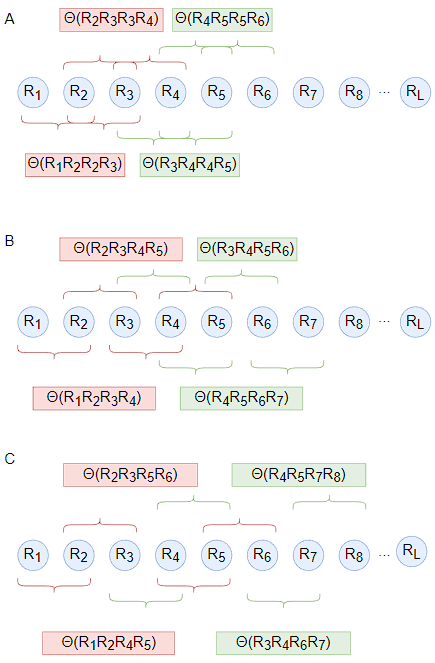
\includegraphics[width=0.65\linewidth]{correlation_di.png}
    \caption{Correlations of dinucleotides along a DNA sequence. Adapted from~\cite{Chen2014PseKNC:Composition}}
    \label{fig:psednc_correlation}
\end{figure}


In Eq.~\ref{eq:PseDNC-thetas}, the parameter $\lambda$ is an integer, representing the highest counted rank (or tier) of the correlation along a DNA sequence, and the correlation function is given by:

\begin{equation}\label{eq:PseDNC-5}
    \Theta(R_{i}R_{i+1}, R_{j}R_{j+1}) = \frac{1}{\mu}\sum_{u=1}^{\mu}[P_{u} (R_{i}R_{i+1}) - P_{u}(R_{j}R_{j+1})]^{2}
\end{equation}

where $\mu$ is the number of local DNA structural properties considered that is equal to 6 in the current study as will be explained later in the text; $P_{u} (R_{i}R_{i+1})$⁠, the numerical value of the \textit{u-th} $(u = 1,2,...,\mu$ DNA local property for the dinucleotide $R_{i}R_{i+1}$ at position $i$ and $P_{u}(R_{j}R_{j+1})$⁠, the corresponding value for the dinucleotide $R_{j}R_{j+1}$ at position $j$.

Multiple lines of evidences have indicated that some local DNA structural properties, i.e. angular parameters (twist, tilt and roll) and translational parameters (shift, slide and rise), have important roles in biological processes, such as protein–DNA interactions, formation of chromosomes and higher-order organization of the genetic material (30–32). Accordingly, these six structural properties might have impact on DNA binding of regulatory proteins, either directly by hampering or favoring complex formation or indirectly through the modulation of the chromatin structures and hence the DNA accessibility (33). Listed in Table
~\ref{tab:original_numerical} are their original numerical values derived from (32) for twist $P_{1}(R_{i}R_{i+1})$⁠, tilt $P_{2}(R_{i}R_{i+1})$⁠, roll $P_{3}(R_{i}R_{i+1})$⁠, shift $P_{4}(R_{i}R_{i+1})$⁠, slide $P_{5}(R_{i}R_{i+1})$⁠, and rise $P_{6}(R_{i}R_{i+1})$⁠, respectively, where $R_{i}R_{i+1}$ represents the 16 possible dinucleotides AA, AC, AG, AT, ..., TT. It was these six DNA local physical structural properties that were to be used as correlation functions to derive the \gls{PseDNC} for the current study. Meanwhile, it is also self-evident why $\mu=6$ in Eq.~\ref{eq:PseDNC-5} for the current case.


\begin{table}[ht]

    \caption{Original numerical values for the six DNA dinucleotide physical structures~\cite{Chen2013IRSpot-PseDNC:Composition}}
    \label{tab:original_numerical}
    
    \centering
    \begin{tabular}{ccccccc}

        \toprule
        \textbf{Dinucleotide} & $P_{1}(R_{i}R_{i+1})$ & $P_{2}(R_{i}R_{i+1})$ & $P_{3}(R_{i}R_{i+1})$ & $P_{4}(R_{i}R_{i+1})$ & $P_{5}(R_{i}R_{i+1})$ & $P_{6}(R_{i}R_{i+1})$\\\midrule

        AA & 0.026  & 0.038 & 0.020 & 1.69 & 2.26 & 7.65 \\\midrule
        AC & 0.036  & 0.038 & 0.023 & 1.32 & 3.03 & 8.93 \\\midrule
        AG & 0.031  & 0.037 & 0.019 & 1.46 & 2.03 & 7.08 \\\midrule
        AT & 0.033  & 0.036 & 0.022 & 1.03 & 3.83 & 9.07 \\\midrule
        CA & 0.016  & 0.025 & 0.017 & 1.07 & 1.78 & 6.38 \\\midrule
        CC & 0.026  & 0.042 & 0.019 & 1.43 & 1.65 & 8.04 \\\midrule
        CG & 0.014  & 0.026 & 0.016 & 1.08 & 2.00 & 6.23 \\\midrule
        CT & 0.031  & 0.037 & 0.019 & 1.46 & 2.03 & 7.08 \\\midrule
        GA & 0.025  & 0.038 & 0.020 & 1.32 & 1.93 & 8.56 \\\midrule
        GC & 0.025  & 0.036 & 0.026 & 1.20 & 2.61 & 9.53 \\\midrule
        GG & 0.026  & 0.042 & 0.019 & 1.43 & 1.65 & 8.04 \\\midrule
        GT & 0.036  & 0.038 & 0.023 & 1.32 & 3.03 & 8.93 \\\midrule
        TA & 0.017  & 0.018 & 0.016 & 0.72 & 1.20 & 6.23 \\\midrule
        TC & 0.025  & 0.038 & 0.020 & 1.32 & 1.93 & 8.56 \\\midrule
        TG & 0.016  & 0.025 & 0.017 & 1.07 & 1.78 & 6.38 \\\midrule
        TT & 0.026  & 0.038 & 0.020 & 1.69 & 2.26 & 7.65 \\

        \bottomrule
    \end{tabular}
\end{table}

Before substituting into Eq.~\ref{eq:PseDNC-5}, the original values as listed in Table~\ref{tab:original_numerical} for $P_{u}(R_{i}R_{i+1} (u = 1,2,...,6)$⁠, they were all subjected to a standard conversion (26), as described by the following equation:

\begin{equation}\label{eq:PseDNC-6}
    P_{u}(R_{i}R_{i+1}) = \frac{P_{u}(R_{i}R_{i+1}) - <P_{u}>}{SD(P_{u})}
\end{equation}

where the symbol $<>$ means taking the average of the quantity therein for 16 different dinucleotides (cf. Eq.~\ref{eq:PseDNC-1-1}), and SD means the corresponding standard deviation. The converted values obtained by Eq.~\ref{eq:PseDNC-6} will have a zero mean value for the 16 different dinucleotides and will remain unchanged if going through the same conversion procedure again. Listed in Table~\ref{tab:normalized_values} are the values of $P_{u}(R_{i}R_{i+1} (u = 1,2,...,6)$ obtained via the standard conversion of Eq.~\ref{eq:PseDNC-6} from those of Table~\ref{tab:original_numerical}.

\begin{table}[ht]

    \caption{The normalized values for the six DNA dinucleotide physical structures
    ~\cite{Chen2013IRSpot-PseDNC:Composition}}
    \label{tab:normalized_values}
    
    \centering
    \begin{tabular}{ccccccc}

        \toprule
        \textbf{Dinucleotide} & $P_{1}(R_{i}R_{i+1})$ & $P_{2}(R_{i}R_{i+1})$ & $P_{3}(R_{i}R_{i+1})$ & $P_{4}(R_{i}R_{i+1})$ & $P_{5}(R_{i}R_{i+1})$ & $P_{6}(R_{i}R_{i+1})$\\\midrule
        
        AA & 0.06  &	0.5 	& 0.27 	& 1.59 	& 0.11 	& -0.11 \\\midrule
        AC & 1.50  &	0.50 	& 0.80 	& 0.13 	& 1.29 	& 1.04 \\\midrule
        AG & 0.78  &	0.36 	& 0.09 	& 0.68 	& -0.24 & -0.62 \\\midrule
        AT & 1.07  &	0.22 	& 0.62 	& -1.02 & 2.51 	& 1.17 \\\midrule
        CA & -1.38 & 	-1.36 	& -0.27 & -0.86 & -0.62 & -1.25 \\\midrule
        CC & 0.06  &	1.08 	& 0.09 	& 0.56 	& -0.82 & 0.24 \\\midrule
        CG & -1.66 & 	-1.22 	& -0.44 & -0.82 & -0.29 & -1.39 \\\midrule
        CT & 0.78  &	0.36 	& 0.09 	& 0.68 	& -0.24 & -0.62 \\\midrule
        GA & -0.08 & 	0.5 	& 0.27 	& 0.13 	& -0.39 & 0.71 \\\midrule
        GC & -0.08 & 	0.22 	& 1.33 	& -0.35 & 0.65 	& 1.59 \\\midrule
        GG & 0.06  &	1.08 	& 0.09 	& 0.56 	& -0.82 & 0.24 \\\midrule
        GT & 1.50  &	0.50 	& 0.80 	& 0.13 	& 1.29 	& 1.04 \\\midrule
        TA & -1.23 & 	-2.37 	& -0.44 & -2.24 & -1.51 & -1.39 \\\midrule
        TC & -0.08 & 	0.5 	& 0.27 	& 0.13 	& -0.39 & 0.71 \\\midrule
        TG & -1.38 & 	-1.36 	& -0.27 & -0.86 & -0.62 & -1.25 \\\midrule
        TT & 0.06  &	0.5 	& 0.27 	& 1.59 	& 0.11 	& -0.11 \\

        \bottomrule
    \end{tabular}
\end{table}

Now we can see that the sequence-order effect of a DNA sequence can be, to some extent, reflected through a set of sequence-correlation factors $\theta_{1},...,\theta_{\lambda}$ as clearly defined by Eq.~\ref{eq:PseDNC-thetas} and \ref{eq:PseDNC-5}. Similar to the procedure as described in (7) for converting the amino acid composition to the PseACC, let us augment the DNC of Eq.~\ref{eq:PseDNC-1-1} to the \gls{PseDNC} as given later in the text

\begin{equation}\label{eq:PseDNC-8}
    D = [d_{1} d_{2} ... d_{16} d_{16+1} ... d_{16+\lambda}]^{T}
\end{equation}

where

\begin{equation}\label{eq:PseDNC-9}
    d_{k} = \begin{cases}\frac{f_{k}}{\sum_{i=1}^{16} f_{i} + w\sum_{j=1}^{\lambda}\theta_{j}} & 1 \le k \le 16\\\frac{w\theta_{k-16}}{\sum_{i=1}^{16} f_{i} + w\sum_{j=1}^{\lambda}\theta_{j}} & 17 \le k \le 16 + \lambda\end{cases}
\end{equation}

where $f_{k} (k = 1,2,...,16)$ are the same as those in Eq.~\ref{eq:PseDNC-1-1}, $\theta_{j} (j = 1,2,...,\lambda$ are given by Eq.~\ref{eq:PseDNC-thetas}, $\lambda$ is the number of the total counted ranks (or tiers) of the correlations along a DNA sequence and $w$ is the weight factor. The concrete values for $\lambda$ and $w$ will be discussed further. Thus, instead of a 16-D (dimensional) vector (cf. Eq.~\ref{eq:PseDNC-1-1}), the DNA sequence is now formulated by a $(16 + \lambda) - D$ vector as shown in Eq.~\ref{eq:PseDNC-8}. It is through the additional $\lambda$ correlation factors that not only considerable global sequence-order effects can be incorporated but the DNA sequences with extreme difference in length can also be converted into a set of feature vectors with a same dimension. The latter is an important pre-requisite for formulating the statistical samples because many powerful classification engines, such as Covariant Discriminant (34,35), Support Vector Machine (SVM) (36) and K-Nearest Neighbor (37–39) algorithms, require the input to be a set of digital vectors with a fixed number of components.

%%%%%%%%%%%%%%%%%%%%%%%%%%%%%%%%%%%%%%%%%%%%%%%%%%%%%%%%%%%%%%%%%%%%%%%%%%%%%%%%%%%%%%%%%%%%%%%%%%%%%%%%%%%%%%%%%%%%%%%%%%%%%%%%%%%%%%%%%%%%%%%%%%%%%%%%%%%%%%%%%%%%%%%%%%%%%%%%%%%%%%%%%%%%%%%%%%%%%%%%%%%%%%%%%%%%%%%%%%%%%%%%%%%%%%%%%%%%%%%%%%%%%%%%%%%%%%%%%%%%%%%%%%%%%%

\subsection{Pseudo K-tupler Composition}

% https://github.com/liufule12/repDNA/blob/master/repDNA/doc/repDNA_manual.pdf

\gls{PseKNC} improved the \gls{PseDNC} approach by incorporating k-tuple nucleotide composition.

Given a DNA sequence D (Eq.~\ref{eq:d-seq}), the feature vector of D is defined:

\begin{equation}\label{eq:PseKNC-feature-vector}
    D = [d_{1}\;d_{2}\;...\;d_{4^{k}}\;d_{4^{k+1}}\;...\;d_{4^{k} + \lambda}]^{T}
\end{equation}

where

\begin{equation}\label{eq:PseKNC-du}
    d_{u} = 
    \begin{cases}
        \frac{f_{u}}{\sum_{i=1}^{4^{k}} f_{i} + w\sum_{j=1}^{\lambda}\theta_{j}} & 1 \le u2 \le 4^{k}
    \\
        \frac{w\theta_{u-4^{k}}}{\sum_{i=1}^{4^{k}} f_{i} + w\sum_{j=1}^{\lambda}\theta_{j}} & 4^{k} \le u \le 4^{k} + \lambda
    
    \end{cases}
\end{equation}

where $\lambda$ is the number of the total counted ranks (or tiers) of the correlations along a DNA sequence; $f_{u}, u\in[1,2,...,4^{k}]$ is the frequency of oligonucleotide that is normalized to $\sum_{i=1}^{4^{k}}f_{i} = 1$; $w$ is a weigth factor; $\theta_{j}$ is given by:

\begin{equation}\label{eq:PseKNC-thetas}
\theta_{j} = \frac{1}{L-j-1} \sum_{i=1}^{L-j-1}\Theta(R_{i}R_{i+1}, R_{i+j}R_{i+j+1}), \;j\in{1,2,...,\lambda;\lambda < L}
\end{equation}

which represents the j-tier structural correlation factor between all the $j^{th}$ most
contiguous dinucleotides. The correlation function $\Theta(R_{i}R_{i+1}, R_{i+j}R_{i+j+1})$ is defined by:

\begin{equation}\label{eq:PseKNC-correlation}
    \Theta(R_{i}R_{i+1}, R_{i+j}R_{i+j+1}) = \frac{1}{\mu}\sum_{v=1}^{\mu}[P_{v} (R_{i}R_{i+1}) - P_{v}(R_{i+j}R_{i+j+1})]^{2}
\end{equation}

where $\mu$ is the number of physicochemical indices, in this study, 6 indices reflecting the local DNA structural properties (Table~\ref{tab:normalized_values}) were employed to generate the \gls{PseKNC} feature vector; $P_{v} (R_{i}R_{i+1})$ represents the numerical value of the v-th physicochemical indices for the dinucleotide $R_{i}R_{i+1}$ at position i and $P_{v} (R_{i+j}R_{i+j+1})$ represents the corresponding value for the dinucleotide $R_{i+j}R_{i+j+1}$ at position i+j.